\section{Fortbewegung und Robotik}

Bionische (biomimetische) Robotik ...

\begin{itemize}
    \item ist inspiriert durch Tiere (weniger Pflanzen).
    \item kopiert nicht, sondern extrahiert Prinzipien.
    \item ist an konkrete Einsatzvorstellungen gekoppelt (Medizin, Militär). 
    \item kombiniert verschiedene Sensordaten nach Vorbild der multimodalen Erfassung von Tieren.
\end{itemize}

\subsection{Inspiration durch Bewegungsmuster}

\begin{enumerate}
    \item Manipulation
    \begin{itemize}
        \item Roboterarm als Abbild des Elefantenrüssels (keine echte Bionik) mit bionischem Greifer nach Vorbild der Fischflosse (echte Bionik) [Festo].
        \begin{center}
            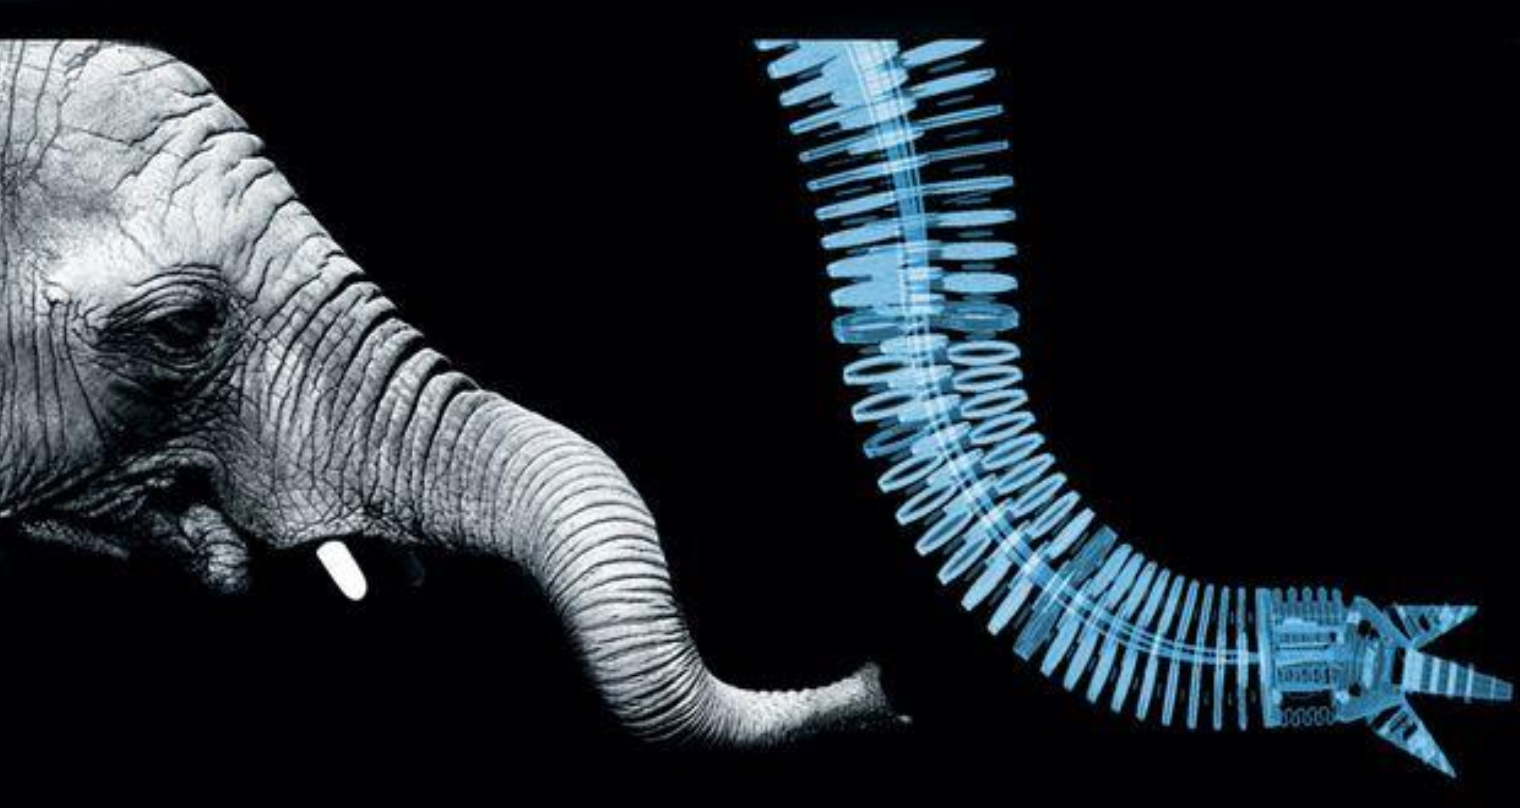
\includegraphics[width=4cm]{lec9/figures/elefant.png}
        \end{center}
        \item FlexShapeGripper: Greifarmkopf inspiriert von der ballistischen Zunge des Chamäleons [Festo].
    \end{itemize}
    \item Kriechen
    \begin{itemize}
        \item Schlangenroboter mit geringer Anzahl an Elementen, damit das System noch gesteuert werden kann (max. 20 Elemente beim Roboter vs. 220 Wirbel bei Boa).
    \end{itemize}
    \item Klettern
    \begin{itemize}
        \item Geckoroboter mit Haftfüßen.
    \end{itemize}
    \item Schwimmen (im Wasser)
    \begin{itemize}
        \item Hairoboter mit geringem Energieverbrauch durch geringen Strömungswiderstand. Haie (die keine Bodenbewohner sind) schwimmen durchgehend, da sie keine Kiemenbewegungen erzeugen können und keine Schwimmblase zum Schweben haben. Daher evolutionär Mikrostruktur der Haut, die Bewuchs verhindert, Reibung reduziert und dadurch eine laminare Strömung und somit einen geringen Energieverbrauch begünstigt. \textbf{\dangersign Detaillierte Funktionsweise?} V-förmige Kämme auf der Haut führen zu spiralförmigen Turbulenzen, dadurch reduzierter Wiederstand in Relation zu chaotischer Turbulenz an normaler Haut. 
        \item Fastskin Schwimmanzüge nach Vorbild der Haihaut [Speedo] .
        \item Riblet-Folie nach Vorbild der Haihaut zur Beklebung von Flugzeugen (Reduktion der Wandreibung ca. 8\%, dadurch ca. 4\% weniger Treibstoffverbrauch).
        \item Schkwal-Torpedo nach Vorbild des Luftblasenschleiers bei Pinguinen mit selbsterneuernder Gashülle. \textbf{\dangersign Funktionsweise?} Pinguin speichert Luftmantel unter Federkleid, die er kontrolliert als Blasenschleier abgeben kann. Dadurch wird der Widerstand verringert, da Zähigkeit von Wasser-Luft-Gemisch geringer ist.
    \end{itemize}
    \item Schimmen (im Sand)
    \begin{itemize}
        \item Roboter nach Vorbild des Sandfischs. Charakteristische Merkmale des Sandfischs sind die keilförmige Schnauze, die rechteckige Körperform, eine scharfe Bauchkante, glatte Schuppen ohne Zwischenraum sowie ein kurzer, kräftiger Schwanz. Abrollwinkel beim Sandfisch (ca. 18 Grad vs. 35 Grad bei Teflon) wird experimentell wie beim Lotus-Effekt mit Sand und toten Tieren ermittelt. Haut ist abriebresistent. Dorsal (auf dem Rücken) befinden sich sägezahnartige Profile mit kammartigen Kanten. Lateral schwach ausgeprägt, ventral nicht vorhanden. Durch diese \textbf{Spikes auf den Strukturen kommt es zu einer Kontaktflächenreduktion} (ein Sahara-Sandkorn berührt ca. 20000 Spikes), welche die \textbf{Reibung reduziert}. Abbrechen der Spikes wird durch spezielle Biegedynamik verhindert. 
        \begin{center}
            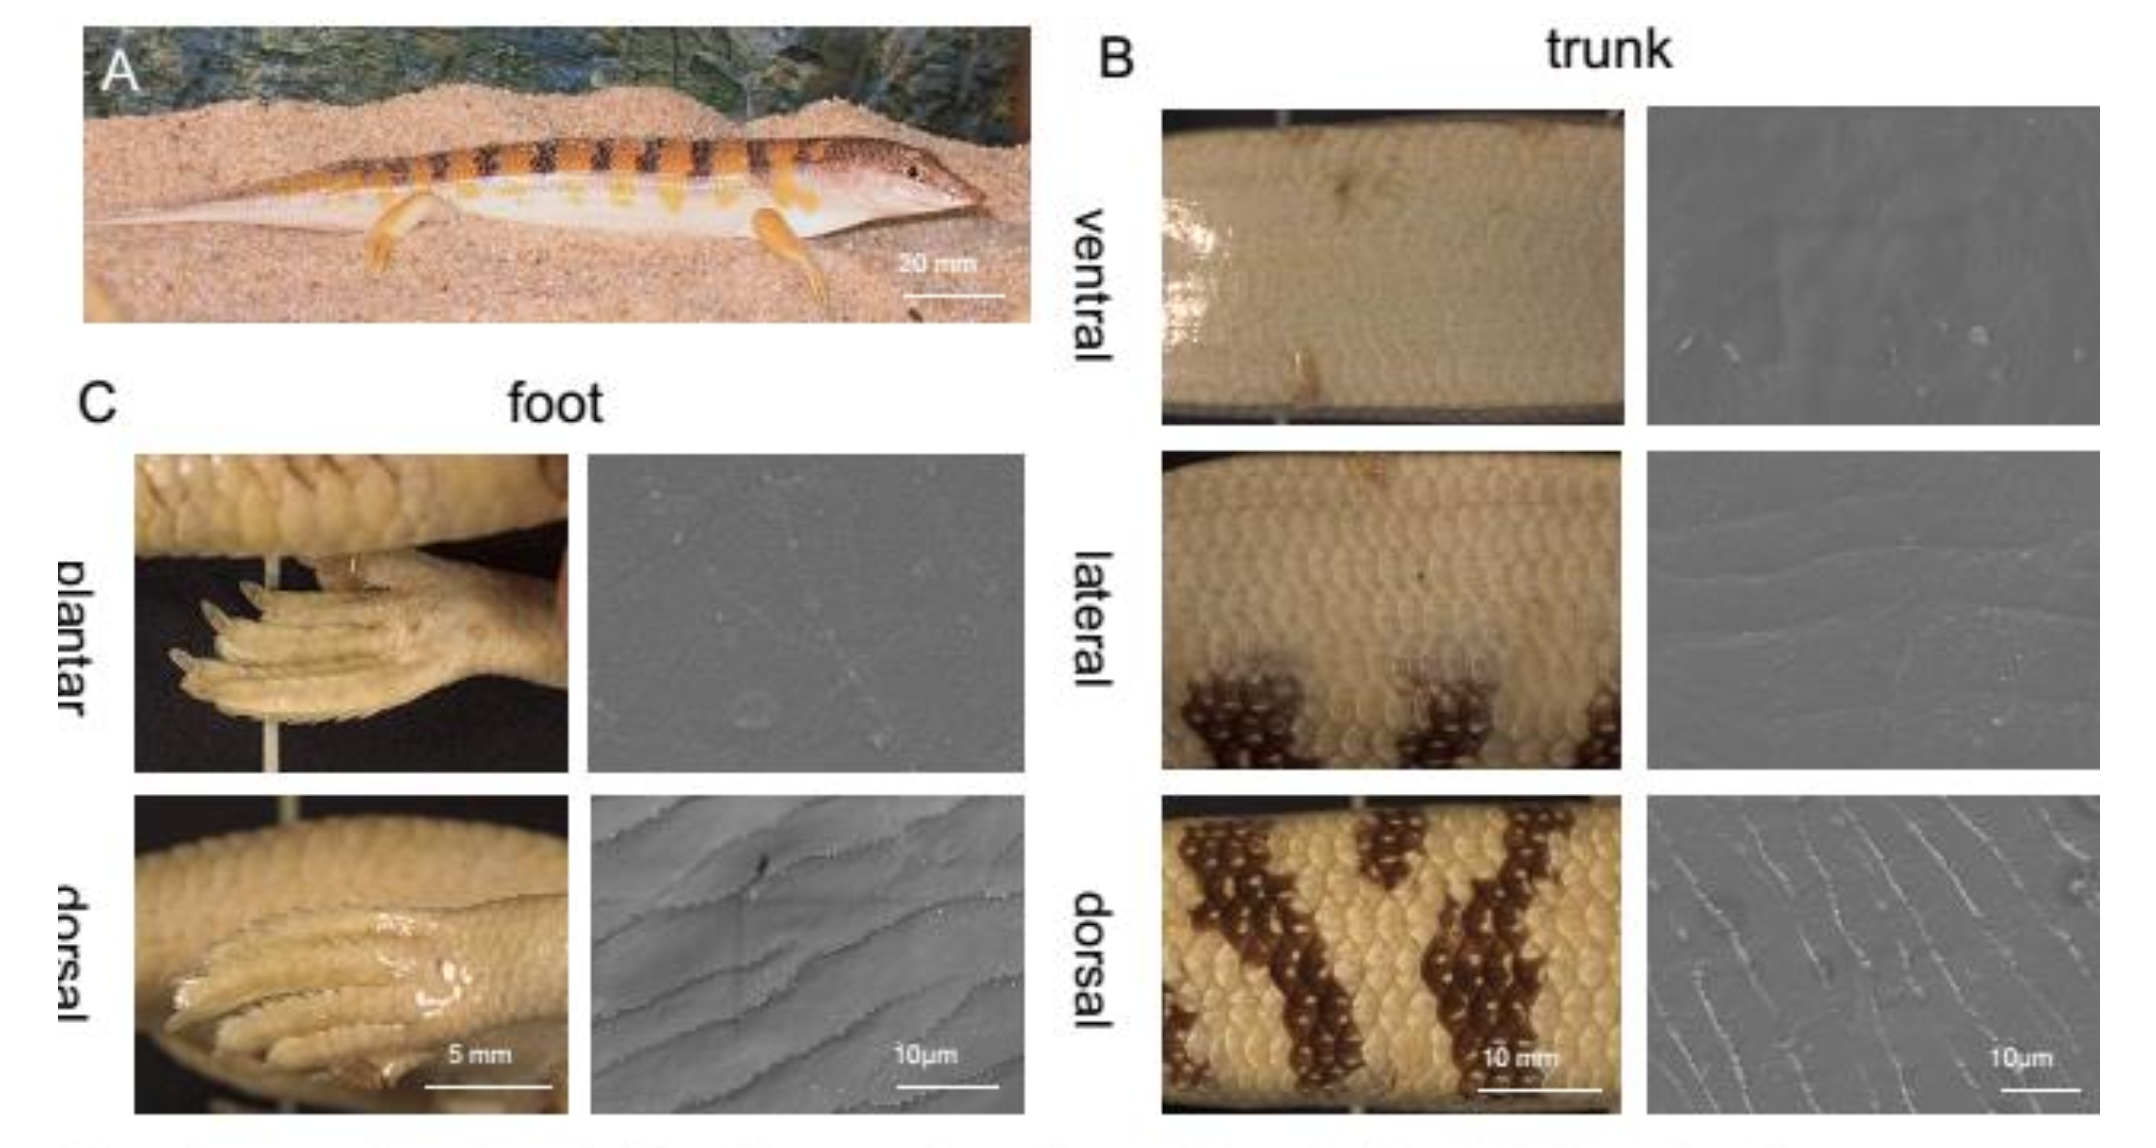
\includegraphics[width=10cm]{lec9/figures/sandfisch.png}
        \end{center}
        \hintsign Eine neuere und anerkannte Hypothese führt den geringen Reibungswiderstand auf die Chemie anstatt der Struktur zurück. Mittels einer SDS-PAGE Chromatographie (Auftrennung eines Stoffgemischs in Einzelbestandteile und Phasen) wurde ermittelt, dass stark glykosylierte $/beta$-Karotione in der Haut des Sandfisch vorhanden sind. Bei Deglykosylierung der Haut (Entfernung des Zuckers) kommt es zu einer starken Zunahme des Reibungswinkels und einer Wechselwirkung mit Sand. \textbf{Glykolsiliertes Kreatin} ist möglicherweise für die geringe Reibung verantwortlich. Dafür spricht, dass die aufgelösten Schuppen des Sandfisches auf Glas aufgebracht einen nahezu identischen Reibungskoeffizienten wie die nicht-aufgelösten Schuppen haben.
        \item Abriebsfester Autolack durch Einbringen der Glykosierten Kreatine in Lacke (siehe Sandfisch).
        \item Abriebfeste Touchscreens, Oberflächen für Sandboards, Antistatik-Belag (geplant).
    \end{itemize}
    \item Fliegen
    \begin{itemize}
        \item Verlängerung der Tragfläche von Flugzeugen nach Vorbild von Albatrossen, um Verhältnis Auftrib zu Umströmung zu verbessern und energiereiche Wirbelbildungen an Flügelenden der Tragflächen zu reduzieren.
        \item Winglets (als fertigungstechnischer Kompromiss zu einem Schlaufenende) nach Vorbild der Auffächerung am Flügelende von Greifvögeln.
        \item Schlagflugmodelle zur Untersuchung von Strömungsverläufen.
        \item Geräuschdämpfung anhand der Untersuchung von Eulenflügeln und deren Turbulenzdämpfungsmechanismen.
    \end{itemize}
    \item Laufen
    \begin{itemize}
        \item Walking Tractor [John Deere], Sechsbeiniger Laufroboter nach Vorbild der Stabheuschrecke \dangersign.
        \item Implementierung von Rückenmarksnetz-werken um motorische Muster des Tieres auf die Größe des Roboters zu skalieren nach Vorbild der CPGs des Salamanders. Das ermöglicht einen hybriden Roboter, welcher sich im Wasser schlängelt und an Land mithilfe seiner Gliedmaßen alternierend laufen kann. \dangersign \textbf{Was sind CPGs? In welchem Teil des Nervensystems
        befinden sich die CPGs bei Wirbeltieren wie zum Beispiel den Salamandern?} (CPG = central pattern generator) sind Ansammlungen von Nervenzellen im Rückenmark, die ohne äußere Aktivierung rhytmisch aktiv sind und Muskeln ansteuern. Unten abgebildete Grafik: Erregung (excitation) in rot und Blockierung (inhibition) in blau bauen sich alternierend auf. Außerdem ist das Aktivierungsmuster zu sehen.
        \begin{center}
            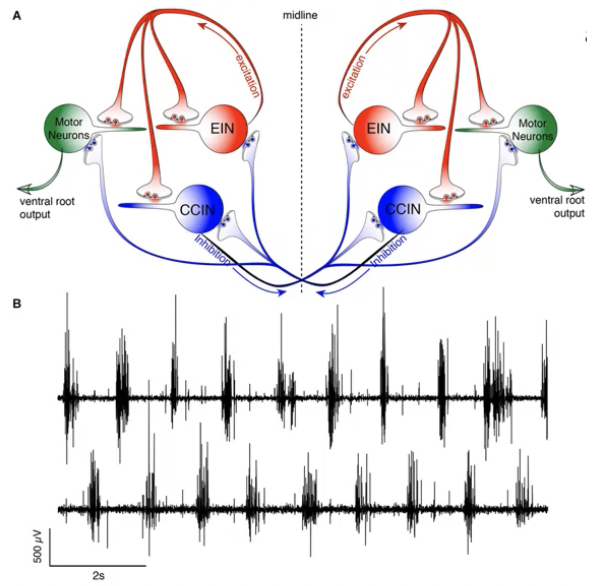
\includegraphics[width=8cm]{lec9/figures/cpg.png}
        \end{center}
        (\dangersign \textit{Welche Strukturen werden bei der Schwimmbewegung des Salamanders von dem CPGs aktiviert?})\\
        (\dangersign \textit{Wie sieht das Aktivierungsmuster der aktivierten Strukturen bei einem schwimmenden Salamander aus?})
        \item Big dog, vierfüßiger Roboter für unwegsames Gelände [Boston Dynamics].
        \item Bionic Kangaroo. Übertragung des Sprungverhaltens durch elastisches Sprungelement nach Vorbild des Känguruu-Schwanzes [Festo].
        \item Zweibeinige Roboter nach Vorbild des Menschen. "Klassische" Robotik, Bein- und Gelenkstellungen mit vielen Sensoren und Stellmontoren kontrolliert, ineffizient. Vereinfachung der Struktur durch "Embodiment".\\
        \begin{center}
            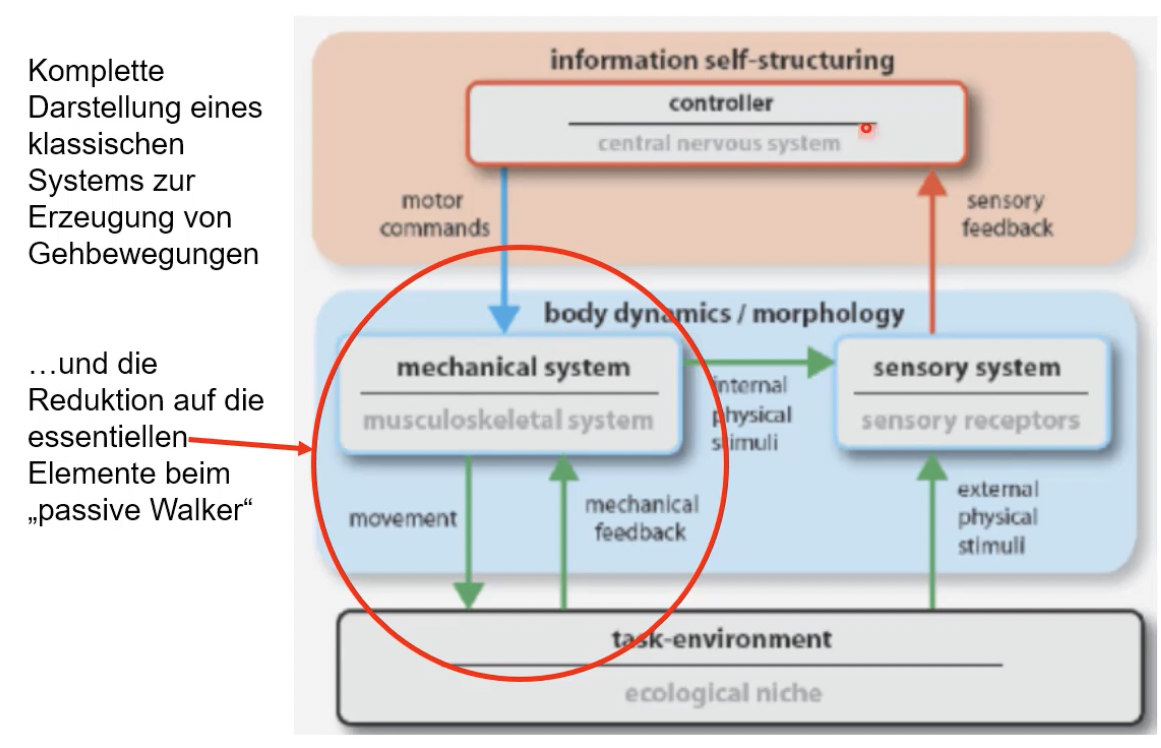
\includegraphics[width=10cm]{lec9/figures/passive-walker.png}
        \end{center}
        (\dangersign \textit{Erklären Sie das Funktionsprinzip eines „passive walker“ aus der bionischen Robotik! Welchen
        wesentlichen Vorteil bringt die Einbeziehung dieses Prinzips bei der Konstruktion von Robotern?})\\
        Prinzip: Rein mechanischer Antrieb ohne Controller, mechanische Umwandlung von potenzieller in kinetische Energie durch Schwerkraft.\\
        Vorteil: Keine kompliziere Steuerung notwendig (Bewegung ohne „Gehirn“ möglich).
    \end{itemize}
\end{enumerate}
